\section{Realne karakteristike operacionog pojačavača}

{Na slici \ref{fig:opampreal} predstavljena je shema realnog operacionog pojačavača.}

\begin{figure}[ht]
    \centering
    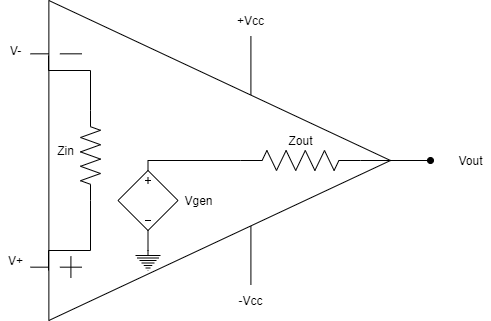
\includegraphics[width=0.6\textwidth]{opampreal.png}
    \caption{Shema realnog operacionog pojačavača.}
    \label{fig:opampreal}
\end{figure}

{Na osnovu slike može se zaključiti da realni operacioni pojačavač ima sledeće karakteristike:}

\begin{enumerate}
    \item {$A_o$ je izuzetno veliko, nije beskonačno.}
    \item {$Z_{in}$ nije beskonačno} - kao posledicu ovoga pojavljuje se struja u ulaznim priključcima operacionog pojačavača (struja polarizacije).
    \item {$Z_{out}$ nije nula, već ima neku relativno malu vrednost} - operacioni pojačavač se ne ponaša kao idealni naponski generator, kao posledica ovoga na izlazu operacionog pojačavača imamo različite izlaze od očekivanih (naponski ofset).
    \item {Karakteristike rada operacionog pojačavača zavise od frekvencije ulaznog signala}.
\end{enumerate}

{Svaka od ovih karakteristika biće detaljno opisana u nastavku teksta.}

\pagebreak
\subsection{Struja polarizacije}

{Struje polarizacije predstavljaju posledicu nesavršenosti realnog operacionog pojačavača. Za razliku od idealnog operacionog pojačavača, kod koga kroz ulazne priključke ne teče struja, kod realnog operacionog pojačavača postoje male ulazne struje koje se nazivaju struje polarizacije. Ove struje mogu izazvati dodatne padove napona na otpornicima u kolu i time dovesti do odstupanja izlaznog napona od njegove idealne vrednosti.}

\begin{figure}[ht]
    \centering
    \begin{circuitikz}[american]
        \begin{scope}
            \ctikzset{tripoles/op amp/width=2.5,   % default 2.5
                    tripoles/op amp/height=2}    % default 2
            \node[op amp] (OA) at (0,0) {};
        \end{scope}
        \draw
            (OA.+) -- ++(-2,0) node[ground] {}
            (OA.-) to [R, l_=$R_1$] ++(-5, 0) to [V, l_=$V_{in}$] ++(0,-1.4) node[ground] {}
            (OA.out) -- ++(1,0) node[right]{$V_{out}$};

        \draw
            (OA.up) -- ++(0,1) node[above]{$+V_{cc}$};

        \draw
            (OA.down) -- ++(0,-1) node[below]{$-V_{cc}$};
        
        \coordinate (topV_minus) at ($(OA.-) + (-0.5, 2.5)$);
        \coordinate (startarrow) at ($(OA.-) + (-1.5, 0)$);

        \draw[->]
            (startarrow) -- ++(1,0) node[midway, above] {$I_1$};

        \draw[->]
            (topV_minus) -- ++(1,0) node[midway, above] {$I_2$};

        \node[circ] at ($(OA.-) + (-0.5,0)$) {};
        \node[below] at ($(OA.-) + (-0.5,0)$) {$V^-$};
        \node[circ] at ($(OA.+) + (-0.5,0)$) {};
        \node[below] at ($(OA.+) + (-0.5,0)$) {$V^+$};
        \node[circ] at (OA.out) {};

        \draw[->]
            ($(OA.-) + (-0.5, 0)$) -- ++(1,0) node[midway, above] {$I_b$};
        \draw[->]   
            ($(OA.+) + (-0.5, 0)$) -- ++(1,0) node[midway, above] {$I_b$};
        \draw
            ($(OA.-) + (-0.5, 0)$) -- (topV_minus) to [R, l=$R_2$] ++(4,0) -- (OA.out);
        
    \end{circuitikz}
    \caption{Izgled operacionog pojačavača u prisustvu struja polarizacije}
    \label{fig:opamp_polarizacije}
\end{figure}

{Sa slike \ref{fig:opamp_polarizacije} može da se zaključi da se sada uvodi još jedna struja, struja polarizacije $I_b$. Pretpostavljeno je da je ova struja jednaka na oba ulaza, odnosno da važi $I_b = I_{b+} = I_{b-}$ , ovo ne mora uvek biti tačno. Sada se iz tačke $V^-$ može napisati I Kirhofov zakon}

\begin{equation}
    I_1 = I_2 + I_b.
    \label{eq:jedan}
\end{equation}

{Izraz za preostale dve struje u kolu ostaje isti, odnosno}

\begin{equation}
    I_1 = \frac{V_{in} - V^-}{R_1} \quad i \quad I_2 = \frac{V^- - V_{out}}{R_2},
\end{equation}

{a zato što je $V^- = V^+ = 0$ dobija se da je izraz za struje zapravo}

\begin{equation}
    I_1 = \frac{V_{in}}{R_1} \quad i \quad I_2 = \frac{- V_{out}}{R_2}.
    \label{eq:dva}
\end{equation}

{Stavljanjem izraza za struje \ref{eq:dva} u jednačinu za I Kirhofov zakon \ref{eq:jedan} dobija se izlaz iz operacionog pojačavača}

\begin{equation}
    \boxed{V_{out} = -\frac{R_2}{R_1}V_{in} + I_bR_2}.
\end{equation}

{Iz jednačine može da se primeti da bi došlo do znatnog odstupanja u vrednosti izlaza operacionog pojačavača usled dodatnog sabiranja sa $I_bR_2$ i baš se u tome ogleda sam problem struja polarizacije.}

{Izraz za neinvertujući pojačavač je sličan te neće biti izvođen već će samo biti tad u svojoj finalnoj formi}

\begin{equation}
    \boxed{V_{out} = V_{in}(1 + \frac{R_2}{R_1}) + I_bR_2}.
\end{equation}

{Kako bi se kompenzovala struja polarizacije neophodno je imati član u izrazu za izlaz operacionog pojačavača $V_{out}$ koji će praktično da negira član $I_bR_2$. Ovo se postiže dodavanjem otpornika $R_3$ na neinvertujući ulaz operacionog pojačavača. Gde sada kolo poprima drugačiji izgled prikazan na slici \ref{fig:opamp_comp}.}

\begin{figure}[ht]
    \centering
    \begin{circuitikz}[american]
        \begin{scope}
            \ctikzset{tripoles/op amp/width=2.5,   % default 2.5
                    tripoles/op amp/height=2}    % default 2
            \node[op amp] (OA) at (0,0) {};
        \end{scope}
        \draw
            (OA.+) -- ++(-2,0) to [R, l_=$R_3$] ++(0, -2) node[ground] {}
            (OA.-) to [R, l_=$R_1$] ++(-5, 0) to [V, l_=$V_{in}$] ++(0,-3.4) node[ground] {}
            (OA.out) -- ++(1,0) node[right]{$V_{out}$};

        \draw
            (OA.up) -- ++(0,1) node[above]{$+V_{cc}$};

        \draw
            (OA.down) -- ++(0,-1) node[below]{$-V_{cc}$};
        
        \coordinate (topV_minus) at ($(OA.-) + (-0.5, 2.5)$);
        \coordinate (startarrow) at ($(OA.-) + (-1.5, 0)$);

        \draw[->]
            (startarrow) -- ++(1,0) node[midway, above] {$I_1$};

        \draw[->]
            (topV_minus) -- ++(1,0) node[midway, above] {$I_2$};

        \node[circ] at ($(OA.-) + (-0.5,0)$) {};
        \node[below] at ($(OA.-) + (-0.5,0)$) {$V^-$};
        \node[circ] at ($(OA.+) + (-0.5,0)$) {};
        \node[below] at ($(OA.+) + (-0.5,0)$) {$V^+$};
        \node[circ] at (OA.out) {};

        \draw[->]
            ($(OA.-) + (-0.5, 0)$) -- ++(1,0) node[midway, above] {$I_b$};
        \draw[->]   
            ($(OA.+) + (-0.5, 0)$) -- ++(1,0) node[midway, above] {$I_b$};
        \draw
            ($(OA.-) + (-0.5, 0)$) -- (topV_minus) to [R, l=$R_2$] ++(4,0) -- (OA.out);
        
    \end{circuitikz}
    \caption{Kompenzacija struja polarizacije}
    \label{fig:opamp_comp}
\end{figure}

{Primenom I Kirhofovog zakona na čvor $V^-$ dobija se izraz}

\begin{equation}
    I_1 = I_2 + I_b,
    \label{cvor}
\end{equation}

{računanjem ostalih struja u kolu dobijaju se izrazi za preostale struje u kolu}

\begin{equation}
    I_1 = \frac{V_{in} - V^-}{R_1} \quad i \quad I_2 = \frac{V^- - V_{out}}{R_2} \quad i \quad I_b = \frac{0 - V^+}{R_3}.
    \label{izrazstruja}
\end{equation}

{Kako se $V^+$ i $V^-$ nalaze na istom potencijalu sledi da je}

\begin{equation}
    V^+ = V^- = -I_bR_3.
    \label{virtuelnamasa}
\end{equation}

{Uvrštanjem izraza za potencijal \ref{virtuelnamasa} u izraz za struju \ref{izrazstruja} i potom uvrtštanjem tih izraza u izraz za I Kirhofov zakon \ref{cvor} dobija se }

\begin{equation}
    \frac{V_{in} + I_bR_3}{R_1} = \frac{-I_bR_3 - V_{out}}{R_2} + I_b.
\end{equation}

{Nakon sređivanja izraza dobija se vrednost za}

\begin{equation}
    V_{out} = -\frac{R_2}{R_1}V_{in} + I_b(R_2 - R_3 -\frac{R_2R_3}{R_1})
\end{equation}

{Kako bi se poništio uticaj struje polarizacije na izlazni napon, potrebno je da član uz $I_b$ bude jednak nuli. Zbog toga mora da važi}

\begin{equation}
R_2-R_3-\frac{R_2R_3}{R_1}=0.
\end{equation}

{Odavde se dobija vrednost otpornika $R_3$
}
\begin{equation}
R_3=\frac{R_1R_2}{R_1+R_2},
\end{equation}

odnosno

\begin{equation}
    \boxed{R_3=R_1\parallel R_2}.
\end{equation}

{Dakle, uticaj struje polarizacije može se kompenzovati izborom otpornika $R_3$ čija je otpornost jednaka paralelnoj vezi otpornika $R_1$ i $R_2$.}

{Princip izvođenja jednačine za kompenzaciju struja polarizacija kod neinvertujućeg operacionog pojačavača je sličan, te neće biti obrađivan.}

\subsection{Naponski ofset}

{Kao i kod struja polarizacija i naponski ofset predstavlja posledicu nesavršenosti realnog operacionog pojačavača. Nastaje zbog nenulte izlazne impedanse operacionog pojačavača. Kod idealnog operacionog pojačavača modeluje se kao naponski generator koji je povezan na neinvertujući ulaz operacionog pojačavača. Primer naponskog ofseta na invertujućem pojačavaču tad je na slici \ref{fig:opamp_offset}.}

\begin{figure}[ht]
    \centering
    \begin{circuitikz}[american]
        \begin{scope}
            \ctikzset{tripoles/op amp/width=2.5,   % default 2.5
                    tripoles/op amp/height=2}    % default 2
            \node[op amp] (OA) at (0,0) {};
        \end{scope}
        \draw
            (OA.+) -- ++(-2,0) to [V, l_=$V_{os}$] ++(0, -2) node[ground] {}
            (OA.-) to [R, l_=$R_1$] ++(-5, 0) to [V, l_=$V_{in}$] ++(0,-3.4) node[ground] {}
            (OA.out) -- ++(1,0) node[right]{$V_{out}$};

        \draw
            (OA.up) -- ++(0,1) node[above]{$+V_{cc}$};

        \draw
            (OA.down) -- ++(0,-1) node[below]{$-V_{cc}$};
        
        \coordinate (topV_minus) at ($(OA.-) + (-0.5, 2.5)$);
        \coordinate (startarrow) at ($(OA.-) + (-1.5, 0)$);

        \draw[->]
            (startarrow) -- ++(1,0) node[midway, above] {$I_1$};

        \draw[->]
            (topV_minus) -- ++(1,0) node[midway, above] {$I_2$};

        \node[circ] at ($(OA.-) + (-0.5,0)$) {};
        \node[below] at ($(OA.-) + (-0.5,0)$) {$V^-$};
        \node[circ] at ($(OA.+) + (-0.5,0)$) {};
        \node[below] at ($(OA.+) + (-0.5,0)$) {$V^+$};
        \node[circ] at (OA.out) {};

        \draw
            ($(OA.-) + (-0.5, 0)$) -- (topV_minus) to [R, l=$R_2$] ++(4,0) -- (OA.out);
        
    \end{circuitikz}
    \caption{Modelovanje naponskog ofseta}
    \label{fig:opamp_offset}
\end{figure}

{Kako se naponski ofset $V_{os}$ modeluje na neinvertujućem ulazu operacionog pojačavača sledi}

\begin{equation}
    V^+ = V_{os} = V^-
    \label{eq:naponvs}
\end{equation}

{Izrazi za struju i dalje ostaju isti, odnosno}

\begin{equation}
    I_1 = \frac{V_{in} - V^-}{R_1} \quad i \quad I_2 = \frac{V^- - V_{out}}{R_2}.
    \label{eq:struje}
\end{equation}

{Gde se nakon uvrštanja izraza \ref{eq:naponvs} u izraz za struje \ref{eq:struje} i njihovog izjednačavanja dobija}

\begin{equation}
    \frac{V_{in} - V_{os}}{R_1} = \frac{V_{os} - V_{out}}{R_2},
\end{equation}

{izražavanjem izlaznog napona kola dobija se}

\begin{equation}
    \boxed{V_{out} = - \frac{R_2}{R_1} V_{in} + (1 + \frac{R_2}{R_1}) V_{os}}.
    \label{vout}
\end{equation}

{Iz jednačine za izlazni napon \ref{vout} se zapravo mogu videti posledice naponskog ofseta na izlaz kola, gde se izlazu dodaje član $(1 + \frac{R_2}{R_1})V_{os}$ koji nepovoljno utiče na izlaz operacionog pojačavača i dovodi do nepredviđenih i nepoželjih izlaza.}

{Izvođenje za neinvertujući operacioni pojačavač je slično, te neće biti obrađivano već će samo biti dato u svojoj finalnoj formi}

\begin{equation}
    \boxed{V_{out} = (1 + \frac{R_2}{R_1})V_{in} + (1 + \frac{R_2}{R_1})V_{os}}.
\end{equation}

{Može se primetiti da i u ovoj izvedbi operacionog pojačavača dolazi do nepoželjnog izobličenja izlazlnog signala istim članom $(1 + \frac{R_2}{R_1})V_{os}$.}

{Slična ideja koja je korišćena kod kompenzacije struja polarizacije koristi se i kod kompenzacije naponskog ofseta, odnosno ideja je oduzeti uticaj naponskog ofseta na izlazu operacionog pojačavača. Ovo se postiže dodavanjem kompenzacionog napona na neinvertujući priključak operacionog pojačavača koji će biti istog inteziteta kao i naponski ofset. Prikaz kompenzacije naponskog ofseta invertujućeg pojačavač prikazan je na slici \ref{fig:opamp_offset_comp}.}

\begin{figure}[ht]
    \centering
    \begin{circuitikz}[american]
        \begin{scope}
            \ctikzset{tripoles/op amp/width=2.5,   % default 2.5
                    tripoles/op amp/height=2}    % default 2
            \node[op amp] (OA) at (0,0) {};
        \end{scope}

        \coordinate (Vos_end) at ($(OA.+) + (-2, -2)$);

        \draw
            (OA.+) -- ++(-2,0) to [V, l_=$V_{os}$] ++(0, -2)
            (OA.-) to [R, l_=$R_1$] ++(-5, 0) to [V, l_=$V_{in}$] ++(0,-3.4) node[ground] {}
            (OA.out) -- ++(1,0) node[right]{$V_{out}$}
            (Vos_end) -- ++(0,-1) to [R, l^=$R_3$, v=$V_{comp}$ ] ++(0,-2) node[ground]{}
            ($(Vos_end) + (0,-1)$) to[R, l=$R_4$] ++(4,0) to[V, l=$V_x$] ++(0, -2) node[ground]{};

        \draw
            (OA.up) -- ++(0,1) node[above]{$+V_{cc}$};

        \draw
            (OA.down) -- ++(0,-1) node[below]{$-V_{cc}$};
        
        \coordinate (topV_minus) at ($(OA.-) + (-0.5, 2.5)$);
        \coordinate (startarrow) at ($(OA.-) + (-1.5, 0)$);

        \draw[->]
            (startarrow) -- ++(1,0) node[midway, above] {$I_1$};

        \draw[->]
            (topV_minus) -- ++(1,0) node[midway, above] {$I_2$};

        \node[circ] at ($(OA.-) + (-0.5,0)$) {};
        \node[below] at ($(OA.-) + (-0.5,0)$) {$V^-$};
        \node[circ] at ($(OA.+) + (-0.5,0)$) {};
        \node[below] at ($(OA.+) + (-0.5,0)$) {$V^+$};
        \node[circ] at (OA.out) {};

        \draw
            ($(OA.-) + (-0.5, 0)$) -- (topV_minus) to [R, l=$R_2$] ++(4,0) -- (OA.out);
        
    \end{circuitikz}
    \caption{Kompenzacija naponskog ofseta}
    \label{fig:opamp_offset_comp}
\end{figure}

\pagebreak
{Kako je neophodno negirati uticaj naponskog ofseta $V_{os}$ mora da važi}

\begin{equation}
    V_{comp} = -V_{os}.
\end{equation}

{Da bi se izračunao napon $V_{comp}$ neophodno je rešiti kolo strujnog razdelnika, gde se nakon njegovog rešavanja dobija vrednost za napon kompenzacije}

\begin{equation}
    \boxed{V_{comp} = \frac{R_3}{R_3 + R_4} V_x}.
\end{equation}

{Kako nam je za napon kompenzacije $V_{comp}$ neophodan negativan napon za naponski generator $V_x$ uzima se napon na $-V_{cc}$, te se za napon kompenzacije dobija sledeći izraz}

\begin{equation}
    V_{comp} = \frac{R_3}{R_3 + R_4} \cdot (-V_{cc}).
\end{equation}

{Kako u izrazu za napon kompenzacije figurišu dve nepoznate vrednosti otpornika $R_3$ i $R_4$, jednu od te dve vrednosti neophodno je proizvoljno odabrati, dok se druga računa. Obrazac za računanje je sledeći, pod pretpostavkom da se proizvoljna vrednost otpornosti uvela za otpornik $R_3$ i za $V_{comp}$ uvedena je vrednost $-V_{os}$}

\begin{equation}
    \boxed{R_4 = \frac{R_3 \cdot (-V_{cc})}{-V_{os}} - R_3}.
\end{equation}

\subsection{Karakteristike operacionog pojačavača zavise od frekvencije ulaznog signala}

{Kao što je prethodno spomenuto izraz za izlazni napon operacionog pojačavača u otvorenoj sprezi je }

\begin{equation}
    V_{out} = A_o \cdot V_{in} = A_o \cdot (V^+ - V^-),
\end{equation}

{gde se smatra da je vrednost za $A_o$ konstanta ili u slučaju operacionog pojačavača u zatvorenoj sprezi zavisna od otpornika $R_1$ i $R_2$. Ovo nije tačno u praksi već pojačanje zavisi od frekvencije ulaznog signala. Sada se pojačanje modeluje kao funkcija prenosa prvog reda, odnosno}

\begin{equation}
    A_o(j\omega) = G(j\omega) = \frac{V_{out}(j\omega)}{V^+(j\omega) - V^-(j\omega)} = \frac{A_o}{1 + j\frac{\omega}{\omega_g}}.
\end{equation}

{Neophodno je razgraničiti pojmove u izrazu, $A_o(j\omega)$ je funkcija prenosa operacionog pojačavača čiji moduo $|A_o(j\omega)|$ određuje pojačanje operacionog pojačavača na određenoj frekveniciji ulaznog signala i čiji argument $arg(A_o(j\omega))$ određuje fazni pomeraj ulaznog signala na određenoj frekvenciji. U funkciji prenosa figuriše i $A_o$ koji predstavlja statičko pojačanje operacionog pojačavača, a $\omega_g$ predstavlja graničnu frekvenciju operacionog pojačavača. Do vrednosti $\omega_g$ se pojačanje smatra konstantnim, nakon $\omega_g$ ono opada.}

{\textit{\textbf{{Primer 1.}}} Pretpostavimo da je $A_o = 1 \,M\frac{V}{V}$, a da je $\omega_g = 20\pi \frac{rad}{s}$. Onda je funkcija prenosa operacionog pojačavača .}

\begin{equation}
    A_o(j\omega) = \frac{10^6}{1 + j\frac{\omega}{20\pi}}
\end{equation}

\begin{figure}[ht]
    \centering

    \begin{minipage}{0.48\textwidth}
        \centering
        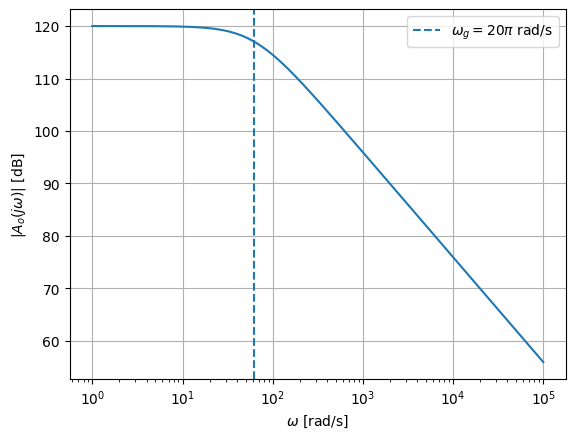
\includegraphics[width=\textwidth]{bode.png}
        \caption{Amplitudska karakteristika}
        \label{fig:amplitudska}
    \end{minipage}
    \hfill
    \begin{minipage}{0.48\textwidth}
        \centering
        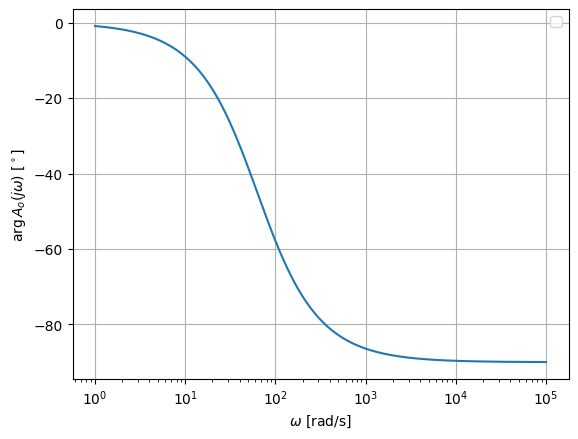
\includegraphics[width=\textwidth]{phase.png}
        \caption{Fazna karakteristika}
        \label{fig:fazna}
    \end{minipage}

\end{figure}